\subsection{Exponential Backoff}\label{cha:expbackoff}
The technique \textit{exponential backoff} is another method used for handling interference. This technique works by incrementing the interval between sending packets, which at some points means the packet will get transferred without any other node interfering. 

For example, if node 1 and 2 are trying to relay data to the main node at the same time, the packet may get corrupt and are therefore not usable. This means that neither node 1 or 2 will get an acknowledgment, and they will both continue sending data. Though, instead of sending data right away, they will wait a small, random but increasing, amount of time before sending again.

A sequence of intervals on a node could be the following: Initial packet sent, wait 1 ms., next package sent, wait 2 ms.,  next package sent, wait 4 ms., next package sent, wait 6 ms. and so on. This continues until the node receives an acknowledgement.

A random number is needed as the nodes needs different intervals. If both nodes have the same interval each time, the packets will continue colliding and the data could never come through. The random number greatly improve the chances that, at some point, one of the sensors will send when the other is waiting. Resulting in the packet being readable.

The used equation to calculate the back off interval, in milliseconds,  is the following:
\begin{equation}
E(c)=2^{c-1}
\end{equation}
Where c is the current attempt number.
We will in addition add a range from 1 to the calculated back off, to ensure we have a  continuous increasing delay to further prevent a interference.

Using this equation to calculate the back off, the delays can be seen on table \ref{cha:expbackoff}.

\begin{table}[]
\centering
\caption{Exponential backoff in milisecounds}
\label{table:expbackoff}
\begin{tabular}{|lllll|}
\hline
Attempt                                                                & Back off range                                         & Best case                                       & Average case                                        & Worst case \\ \hline
\rowcolor[HTML]{EFEFEF} 
\multicolumn{1}{|l|}{\cellcolor[HTML]{EFEFEF}1}                        & \multicolumn{1}{l|}{\cellcolor[HTML]{EFEFEF}1 to 1}    & \multicolumn{1}{l|}{\cellcolor[HTML]{EFEFEF}1}  & \multicolumn{1}{l|}{\cellcolor[HTML]{EFEFEF}1}      & 1          \\
\multicolumn{1}{|l|}{2}                                                & \multicolumn{1}{l|}{1 to 2}                            & \multicolumn{1}{l|}{1}                          & \multicolumn{1}{l|}{1.5}                            & 2          \\
\rowcolor[HTML]{EFEFEF} 
\multicolumn{1}{|l|}{\cellcolor[HTML]{EFEFEF}{\color[HTML]{333333} 3}} & \multicolumn{1}{l|}{\cellcolor[HTML]{EFEFEF}1 to 4}    & \multicolumn{1}{l|}{\cellcolor[HTML]{EFEFEF}2}  & \multicolumn{1}{l|}{\cellcolor[HTML]{EFEFEF}3.5}    & 7          \\
\multicolumn{1}{|l|}{4}                                                & \multicolumn{1}{l|}{1 to 8}                            & \multicolumn{1}{l|}{3}                          & \multicolumn{1}{l|}{7.5}                            & 15         \\
\rowcolor[HTML]{EFEFEF} 
\multicolumn{1}{|l|}{\cellcolor[HTML]{EFEFEF}5}                        & \multicolumn{1}{l|}{\cellcolor[HTML]{EFEFEF}1 to 16}   & \multicolumn{1}{l|}{\cellcolor[HTML]{EFEFEF}4}  & \multicolumn{1}{l|}{\cellcolor[HTML]{EFEFEF}15.5}   & 31         \\
\multicolumn{1}{|l|}{6}                                                & \multicolumn{1}{l|}{1 to 32}                           & \multicolumn{1}{l|}{5}                          & \multicolumn{1}{l|}{31.5}                           & 63         \\
\rowcolor[HTML]{EFEFEF} 
\multicolumn{1}{|l|}{\cellcolor[HTML]{EFEFEF}7}                        & \multicolumn{1}{l|}{\cellcolor[HTML]{EFEFEF}1 to 64}   & \multicolumn{1}{l|}{\cellcolor[HTML]{EFEFEF}6}  & \multicolumn{1}{l|}{\cellcolor[HTML]{EFEFEF}63.5}   & 127        \\
\multicolumn{1}{|l|}{8}                                                & \multicolumn{1}{l|}{1 to 128}                          & \multicolumn{1}{l|}{7}                          & \multicolumn{1}{l|}{127.5}                          & 255        \\
\rowcolor[HTML]{EFEFEF} 
\multicolumn{1}{|l|}{\cellcolor[HTML]{EFEFEF}9}                        & \multicolumn{1}{l|}{\cellcolor[HTML]{EFEFEF}1 to 256}  & \multicolumn{1}{l|}{\cellcolor[HTML]{EFEFEF}8}  & \multicolumn{1}{l|}{\cellcolor[HTML]{EFEFEF}255.5}  & 511        \\
\multicolumn{1}{|l|}{10}                                               & \multicolumn{1}{l|}{1 to 512}                          & \multicolumn{1}{l|}{9}                          & \multicolumn{1}{l|}{511.5}                          & 1023       \\
\rowcolor[HTML]{EFEFEF} 
\multicolumn{1}{|l|}{\cellcolor[HTML]{EFEFEF}11}                       & \multicolumn{1}{l|}{\cellcolor[HTML]{EFEFEF}1 to 1024} & \multicolumn{1}{l|}{\cellcolor[HTML]{EFEFEF}10} & \multicolumn{1}{l|}{\cellcolor[HTML]{EFEFEF}1023.5} & 2047       \\ \hline
\end{tabular}
\end{table}

Compared on \ref{fig:expbackoff} it can be noted how the exponential backoff is ever exponential increasing.
Which is why there will be implemented a limit to the backoff delay, to avoid very long waiting in extreme cases.

\begin{figure}[H]\label{fig:expbackoff}
\centering
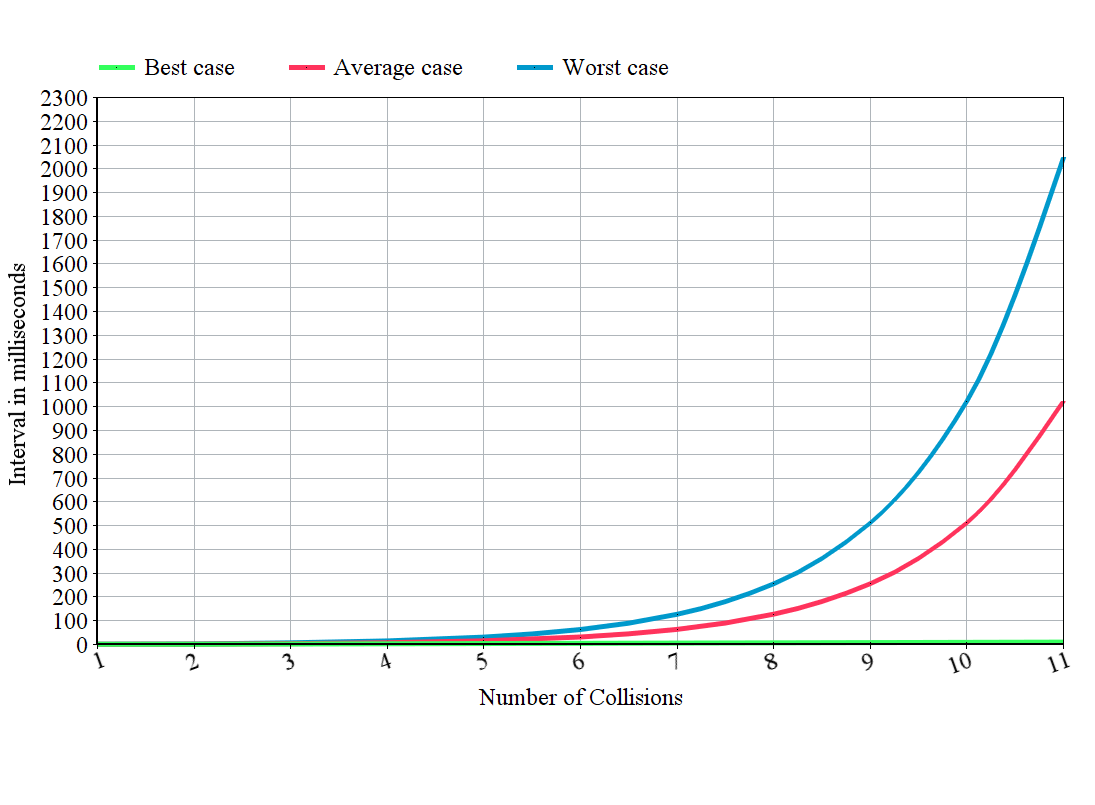
\includegraphics{figures/backoff.PNG}
\caption{Exponential backoff in milisecounds}
\label{fig:expbackoff}
\end{figure}
